\documentclass[10pt,twocolumn]{article}
\usepackage[letterpaper,margin=0.72in,columnsep=0.25in]{geometry}
\usepackage{amsmath,amssymb,graphicx,booktabs,microtype,url}
\usepackage[font=small,labelfont=bf]{caption}
\usepackage[hidelinks]{hyperref}
\setlength{\parindent}{1em}
\setlength{\parskip}{2pt}
\setlength{\textfloatsep}{12pt}
\setlength{\dbltextfloatsep}{12pt}
\raggedbottom
\newcommand{\LowCEAcc}{35.02}
\newcommand{\LowCEFone}{26.39}
\newcommand{\LowCEMAE}{0.990}
\newcommand{\LowCESevere}{26.05}
\newcommand{\LowCEECE}{1.74}
\newcommand{\LowCENLL}{1.483}
\newcommand{\LowCEBrier}{0.749}
\newcommand{\LowCERPS}{0.165}
\newcommand{\LowCECentral}{7.92}
\newcommand{\LowCETSAcc}{35.02}
\newcommand{\LowCETSFone}{26.39}
\newcommand{\LowCETSMAE}{0.990}
\newcommand{\LowCETSSevere}{26.05}
\newcommand{\LowCETSECE}{2.03}
\newcommand{\LowCETSNLL}{1.482}
\newcommand{\LowCETSBrier}{0.749}
\newcommand{\LowCETSRPS}{0.164}
\newcommand{\LowCETSCentral}{7.92}
\newcommand{\LowCEMAEAcc}{35.11}
\newcommand{\LowCEMAEFone}{28.12}
\newcommand{\LowCEMAEMAE}{0.988}
\newcommand{\LowCEMAESevere}{25.84}
\newcommand{\LowCEMAEECE}{4.53}
\newcommand{\LowCEMAENLL}{1.491}
\newcommand{\LowCEMAEBrier}{0.754}
\newcommand{\LowCEMAERPS}{0.163}
\newcommand{\LowCEMAECentral}{9.82}
\newcommand{\LowMedianAcc}{27.60}
\newcommand{\LowMedianFone}{20.03}
\newcommand{\LowMedianMAE}{0.955}
\newcommand{\LowMedianSevere}{21.49}
\newcommand{\LowMedianECE}{1.74}
\newcommand{\LowMedianNLL}{1.483}
\newcommand{\LowMedianBrier}{0.749}
\newcommand{\LowMedianRPS}{0.165}
\newcommand{\LowMedianCentral}{60.95}
\newcommand{\LowCumAcc}{35.91}
\newcommand{\LowCumFone}{24.69}
\newcommand{\LowCumMAE}{0.939}
\newcommand{\LowCumSevere}{23.09}
\newcommand{\LowCumECE}{1.81}
\newcommand{\LowCumNLL}{1.485}
\newcommand{\LowCumBrier}{0.748}
\newcommand{\LowCumRPS}{0.164}
\newcommand{\LowCumCentral}{9.52}
\newcommand{\LowDPoneAcc}{35.38}
\newcommand{\LowDPoneFone}{26.51}
\newcommand{\LowDPoneMAE}{0.976}
\newcommand{\LowDPoneSevere}{25.35}
\newcommand{\LowDPoneECE}{2.67}
\newcommand{\LowDPoneNLL}{1.479}
\newcommand{\LowDPoneBrier}{0.749}
\newcommand{\LowDPoneRPS}{0.163}
\newcommand{\LowDPoneCentral}{9.13}
\newcommand{\LowDPtwoAcc}{35.26}
\newcommand{\LowDPtwoFone}{26.13}
\newcommand{\LowDPtwoMAE}{0.977}
\newcommand{\LowDPtwoSevere}{25.34}
\newcommand{\LowDPtwoECE}{2.14}
\newcommand{\LowDPtwoNLL}{1.480}
\newcommand{\LowDPtwoBrier}{0.749}
\newcommand{\LowDPtwoRPS}{0.164}
\newcommand{\LowDPtwoCentral}{9.03}
\newcommand{\LowDPtwoTSAcc}{35.26}
\newcommand{\LowDPtwoTSFone}{26.13}
\newcommand{\LowDPtwoTSMAE}{0.977}
\newcommand{\LowDPtwoTSSevere}{25.34}
\newcommand{\LowDPtwoTSECE}{1.78}
\newcommand{\LowDPtwoTSNLL}{1.479}
\newcommand{\LowDPtwoTSBrier}{0.749}
\newcommand{\LowDPtwoTSRPS}{0.163}
\newcommand{\LowDPtwoTSCentral}{9.03}
\newcommand{\LowDPNLLAcc}{35.17}
\newcommand{\LowDPNLLFone}{25.54}
\newcommand{\LowDPNLLMAE}{0.968}
\newcommand{\LowDPNLLSevere}{24.77}
\newcommand{\LowDPNLLECE}{2.00}
\newcommand{\LowDPNLLNLL}{1.478}
\newcommand{\LowDPNLLBrier}{0.749}
\newcommand{\LowDPNLLRPS}{0.163}
\newcommand{\LowDPNLLCentral}{10.11}
\newcommand{\LowDPfixedAcc}{35.22}
\newcommand{\LowDPfixedFone}{26.26}
\newcommand{\LowDPfixedMAE}{0.980}
\newcommand{\LowDPfixedSevere}{25.54}
\newcommand{\LowDPfixedECE}{2.04}
\newcommand{\LowDPfixedNLL}{1.480}
\newcommand{\LowDPfixedBrier}{0.749}
\newcommand{\LowDPfixedRPS}{0.164}
\newcommand{\LowDPfixedCentral}{8.66}
\newcommand{\LowLSAcc}{35.07}
\newcommand{\LowLSFone}{26.44}
\newcommand{\LowLSMAE}{0.989}
\newcommand{\LowLSSevere}{26.02}
\newcommand{\LowLSECE}{2.90}
\newcommand{\LowLSNLL}{1.487}
\newcommand{\LowLSBrier}{0.751}
\newcommand{\LowLSRPS}{0.166}
\newcommand{\LowLSCentral}{7.86}
\newcommand{\LowLSTSAcc}{35.07}
\newcommand{\LowLSTSFone}{26.44}
\newcommand{\LowLSTSMAE}{0.989}
\newcommand{\LowLSTSSevere}{26.02}
\newcommand{\LowLSTSECE}{2.07}
\newcommand{\LowLSTSNLL}{1.481}
\newcommand{\LowLSTSBrier}{0.749}
\newcommand{\LowLSTSRPS}{0.164}
\newcommand{\LowLSTSCentral}{7.86}
\newcommand{\LowNBAcc}{34.78}
\newcommand{\LowNBFone}{19.38}
\newcommand{\LowNBMAE}{0.985}
\newcommand{\LowNBSevere}{25.08}
\newcommand{\LowNBECE}{2.33}
\newcommand{\LowNBNLL}{1.523}
\newcommand{\LowNBBrier}{0.765}
\newcommand{\LowNBRPS}{0.169}
\newcommand{\LowNBCentral}{1.22}
\newcommand{\LowOLLAcc}{35.02}
\newcommand{\LowOLLFone}{21.89}
\newcommand{\LowOLLMAE}{0.931}
\newcommand{\LowOLLSevere}{22.14}
\newcommand{\LowOLLECE}{10.88}
\newcommand{\LowOLLNLL}{9.936}
\newcommand{\LowOLLBrier}{0.844}
\newcommand{\LowOLLRPS}{0.180}
\newcommand{\LowOLLCentral}{10.51}
\newcommand{\LowOLLTSAcc}{35.02}
\newcommand{\LowOLLTSFone}{21.89}
\newcommand{\LowOLLTSMAE}{0.931}
\newcommand{\LowOLLTSSevere}{22.14}
\newcommand{\LowOLLTSECE}{5.67}
\newcommand{\LowOLLTSNLL}{1.683}
\newcommand{\LowOLLTSBrier}{0.814}
\newcommand{\LowOLLTSRPS}{0.190}
\newcommand{\LowOLLTSCentral}{10.51}
\newcommand{\LowOLLregAcc}{18.48}
\newcommand{\LowOLLregFone}{7.43}
\newcommand{\LowOLLregMAE}{1.108}
\newcommand{\LowOLLregSevere}{29.23}
\newcommand{\LowOLLregECE}{20.93}
\newcommand{\LowOLLregNLL}{6.512}
\newcommand{\LowOLLregBrier}{0.886}
\newcommand{\LowOLLregRPS}{0.202}
\newcommand{\LowOLLregCentral}{96.71}
\newcommand{\LowOLLregTSAcc}{18.48}
\newcommand{\LowOLLregTSFone}{7.43}
\newcommand{\LowOLLregTSMAE}{1.108}
\newcommand{\LowOLLregTSSevere}{29.23}
\newcommand{\LowOLLregTSECE}{7.88}
\newcommand{\LowOLLregTSNLL}{1.613}
\newcommand{\LowOLLregTSBrier}{0.800}
\newcommand{\LowOLLregTSRPS}{0.188}
\newcommand{\LowOLLregTSCentral}{96.71}
\newcommand{\FullCEAcc}{40.77}
\newcommand{\FullCEFone}{35.06}
\newcommand{\FullCEMAE}{0.830}
\newcommand{\FullCESevere}{18.82}
\newcommand{\FullCEECE}{3.37}
\newcommand{\FullCENLL}{1.375}
\newcommand{\FullCEBrier}{0.705}
\newcommand{\FullCERPS}{0.144}
\newcommand{\FullCECentral}{10.09}
\newcommand{\FullCETSAcc}{40.77}
\newcommand{\FullCETSFone}{35.06}
\newcommand{\FullCETSMAE}{0.830}
\newcommand{\FullCETSSevere}{18.82}
\newcommand{\FullCETSECE}{2.37}
\newcommand{\FullCETSNLL}{1.369}
\newcommand{\FullCETSBrier}{0.704}
\newcommand{\FullCETSRPS}{0.141}
\newcommand{\FullCETSCentral}{10.09}
\newcommand{\FullCEMAEAcc}{40.71}
\newcommand{\FullCEMAEFone}{36.05}
\newcommand{\FullCEMAEMAE}{0.829}
\newcommand{\FullCEMAESevere}{18.55}
\newcommand{\FullCEMAEECE}{5.26}
\newcommand{\FullCEMAENLL}{1.381}
\newcommand{\FullCEMAEBrier}{0.710}
\newcommand{\FullCEMAERPS}{0.141}
\newcommand{\FullCEMAECentral}{11.75}
\newcommand{\FullMedianAcc}{35.38}
\newcommand{\FullMedianFone}{27.92}
\newcommand{\FullMedianMAE}{0.802}
\newcommand{\FullMedianSevere}{14.21}
\newcommand{\FullMedianECE}{3.37}
\newcommand{\FullMedianNLL}{1.375}
\newcommand{\FullMedianBrier}{0.705}
\newcommand{\FullMedianRPS}{0.144}
\newcommand{\FullMedianCentral}{41.99}
\newcommand{\FullCumAcc}{41.18}
\newcommand{\FullCumFone}{32.93}
\newcommand{\FullCumMAE}{0.783}
\newcommand{\FullCumSevere}{15.70}
\newcommand{\FullCumECE}{2.53}
\newcommand{\FullCumNLL}{1.370}
\newcommand{\FullCumBrier}{0.703}
\newcommand{\FullCumRPS}{0.143}
\newcommand{\FullCumCentral}{11.54}
\newcommand{\FullDPoneAcc}{40.95}
\newcommand{\FullDPoneFone}{34.98}
\newcommand{\FullDPoneMAE}{0.819}
\newcommand{\FullDPoneSevere}{18.28}
\newcommand{\FullDPoneECE}{3.02}
\newcommand{\FullDPoneNLL}{1.363}
\newcommand{\FullDPoneBrier}{0.702}
\newcommand{\FullDPoneRPS}{0.141}
\newcommand{\FullDPoneCentral}{10.77}
\newcommand{\FullDPtwoAcc}{41.04}
\newcommand{\FullDPtwoFone}{34.27}
\newcommand{\FullDPtwoMAE}{0.803}
\newcommand{\FullDPtwoSevere}{17.19}
\newcommand{\FullDPtwoECE}{2.14}
\newcommand{\FullDPtwoNLL}{1.359}
\newcommand{\FullDPtwoBrier}{0.702}
\newcommand{\FullDPtwoRPS}{0.140}
\newcommand{\FullDPtwoCentral}{11.99}
\newcommand{\FullDPtwoTSAcc}{41.04}
\newcommand{\FullDPtwoTSFone}{34.27}
\newcommand{\FullDPtwoTSMAE}{0.803}
\newcommand{\FullDPtwoTSSevere}{17.19}
\newcommand{\FullDPtwoTSECE}{2.23}
\newcommand{\FullDPtwoTSNLL}{1.358}
\newcommand{\FullDPtwoTSBrier}{0.702}
\newcommand{\FullDPtwoTSRPS}{0.140}
\newcommand{\FullDPtwoTSCentral}{11.99}
\newcommand{\FullDPNLLAcc}{41.04}
\newcommand{\FullDPNLLFone}{34.27}
\newcommand{\FullDPNLLMAE}{0.803}
\newcommand{\FullDPNLLSevere}{17.19}
\newcommand{\FullDPNLLECE}{2.14}
\newcommand{\FullDPNLLNLL}{1.359}
\newcommand{\FullDPNLLBrier}{0.702}
\newcommand{\FullDPNLLRPS}{0.140}
\newcommand{\FullDPNLLCentral}{11.99}
\newcommand{\FullDPfixedAcc}{41.00}
\newcommand{\FullDPfixedFone}{35.00}
\newcommand{\FullDPfixedMAE}{0.822}
\newcommand{\FullDPfixedSevere}{18.46}
\newcommand{\FullDPfixedECE}{3.18}
\newcommand{\FullDPfixedNLL}{1.369}
\newcommand{\FullDPfixedBrier}{0.704}
\newcommand{\FullDPfixedRPS}{0.143}
\newcommand{\FullDPfixedCentral}{10.54}
\newcommand{\FullLSAcc}{40.95}
\newcommand{\FullLSFone}{35.25}
\newcommand{\FullLSMAE}{0.827}
\newcommand{\FullLSSevere}{18.78}
\newcommand{\FullLSECE}{4.44}
\newcommand{\FullLSNLL}{1.385}
\newcommand{\FullLSBrier}{0.708}
\newcommand{\FullLSRPS}{0.146}
\newcommand{\FullLSCentral}{9.91}
\newcommand{\FullLSTSAcc}{40.95}
\newcommand{\FullLSTSFone}{35.25}
\newcommand{\FullLSTSMAE}{0.827}
\newcommand{\FullLSTSSevere}{18.78}
\newcommand{\FullLSTSECE}{2.58}
\newcommand{\FullLSTSNLL}{1.369}
\newcommand{\FullLSTSBrier}{0.704}
\newcommand{\FullLSTSRPS}{0.141}
\newcommand{\FullLSTSCentral}{9.91}
\newcommand{\FullNBAcc}{39.97}
\newcommand{\FullNBFone}{32.35}
\newcommand{\FullNBMAE}{0.831}
\newcommand{\FullNBSevere}{18.19}
\newcommand{\FullNBECE}{6.28}
\newcommand{\FullNBNLL}{1.414}
\newcommand{\FullNBBrier}{0.723}
\newcommand{\FullNBRPS}{0.142}
\newcommand{\FullNBCentral}{9.85}
\newcommand{\FullOLLAcc}{38.37}
\newcommand{\FullOLLFone}{24.97}
\newcommand{\FullOLLMAE}{0.790}
\newcommand{\FullOLLSevere}{14.34}
\newcommand{\FullOLLECE}{12.07}
\newcommand{\FullOLLNLL}{11.713}
\newcommand{\FullOLLBrier}{0.828}
\newcommand{\FullOLLRPS}{0.166}
\newcommand{\FullOLLCentral}{15.11}
\newcommand{\FullOLLTSAcc}{38.37}
\newcommand{\FullOLLTSFone}{24.97}
\newcommand{\FullOLLTSMAE}{0.790}
\newcommand{\FullOLLTSSevere}{14.34}
\newcommand{\FullOLLTSECE}{8.42}
\newcommand{\FullOLLTSNLL}{1.698}
\newcommand{\FullOLLTSBrier}{0.816}
\newcommand{\FullOLLTSRPS}{0.190}
\newcommand{\FullOLLTSCentral}{15.11}
\newcommand{\FullOLLregAcc}{30.00}
\newcommand{\FullOLLregFone}{21.17}
\newcommand{\FullOLLregMAE}{0.887}
\newcommand{\FullOLLregSevere}{17.24}
\newcommand{\FullOLLregECE}{8.77}
\newcommand{\FullOLLregNLL}{5.649}
\newcommand{\FullOLLregBrier}{0.856}
\newcommand{\FullOLLregRPS}{0.189}
\newcommand{\FullOLLregCentral}{54.98}
\newcommand{\FullOLLregTSAcc}{30.00}
\newcommand{\FullOLLregTSFone}{21.17}
\newcommand{\FullOLLregTSMAE}{0.887}
\newcommand{\FullOLLregTSSevere}{17.24}
\newcommand{\FullOLLregTSECE}{4.45}
\newcommand{\FullOLLregTSNLL}{1.600}
\newcommand{\FullOLLregTSBrier}{0.795}
\newcommand{\FullOLLregTSRPS}{0.187}
\newcommand{\FullOLLregTSCentral}{54.98}
\newcommand{\TrainCount}{8531}
\newcommand{\DevCount}{1100}
\newcommand{\TestCount}{2210}
\newcommand{\RemovedCount}{14}

\title{Ordinal Error and Probability Calibration in\ Lightweight Five-Level Sentiment Classification}
\author{Karthikeya Kumar\\
\small Aditya University, Dept of AIML\\
\small \href{mailto:karthikeya2k7@zohomail.in}{karthikeya2k7@zohomail.in}}
\date{6 October 2026}

\begin{document}
\maketitle
\begin{abstract}
Sentiment labels often have an order, but reducing the distance between predicted and true labels need not produce reliable probabilities. We investigate this distinction using CPU-trained TF-IDF classifiers on the five-level Stanford Sentiment Treebank. We compare nominal cross-entropy, distance-penalized cross-entropy, ordinal log-loss, cumulative logistic regression, label smoothing, temperature scaling, and a posterior-median decision rule. Two training budgets and three development splits are evaluated without using test labels for model selection. With the full training set, a validation-selected quadratic distance penalty reduces mean absolute error from \FullCEMAE{} to \FullDPtwoMAE{} and errors of at least two levels from \FullCESevere\% to \FullDPtwoSevere\%. Its 15-bin calibration error decreases from \FullCEECE\% to \FullDPtwoECE\%, but cumulative logistic regression achieves lower mean absolute error (\FullCumMAE{}). At the smaller training budget, the penalty has higher calibration error than cross-entropy. Standalone ordinal log-loss suppresses extreme-label predictions and has poor negative log-likelihood in this representation. Secondary controls and a loss-risk diagnostic help explain these findings. The results support evaluating ordinal decision quality and probability calibration separately, rather than assuming that a distance-aware objective improves both.
\end{abstract}

\section{Introduction}
Sentiment classification is often introduced as a positive-versus-negative decision. A five-level task is more demanding: a sentence may be strongly negative, moderately negative, neutral, moderately positive, or strongly positive. Misclassifying a strongly negative sentence as moderately negative has a different interpretation from labeling it strongly positive. Accuracy counts both errors equally, whereas an ordinal metric distinguishes them. In review-analysis applications, this distinction can affect how a system prioritizes feedback or summarizes a distribution of opinions.

The probability attached to a prediction is another concern. A classifier that reduces severe mistakes may still assign very low probability to the correct class. Conversely, a classifier can improve its probability estimates while leaving its predicted labels unchanged. A practical evaluation should therefore consider both the action taken by the model and the uncertainty represented by its output distribution.

Ordinal sentiment modeling is not a new problem. The Stanford Sentiment Treebank provides an established five-level task \cite{socher2013}, and ordinal log-loss has already been studied on this dataset \cite{castagnos2022}. The Multilingual Amazon Reviews Corpus also explicitly motivates mean absolute error for ordered review ratings \cite{keung2020}. These precedents rule out presenting a distance penalty alone as a new research contribution. Our study instead asks a narrower empirical question: \emph{in a lightweight sparse classifier, does adding expected ordinal distance to cross-entropy improve both severe-error behavior and probability quality?}

This question is suitable for limited computational resources because the representation and classification head can be held fixed while only the objective changes. It also makes negative results informative. We do not fine-tune a pretrained language model or compare our accuracy with transformer benchmarks. Our focus is the relationship among losses, decision rules, and evaluation metrics within a controlled CPU setting.

We test two primary hypotheses. First, a validation-selected quadratic distance penalty should reduce argmax mean absolute error and the frequency of errors spanning at least two levels. Second, it should improve calibration error and negative log-likelihood. The hypotheses are evaluated separately because they need not agree. Temperature scaling and posterior-median decisions provide additional controls: the former changes probabilities without changing argmax labels, while the latter changes decisions without retraining the probability model.

The contribution is a reproducible comparison with explicit evidence boundaries. We preserve official sentence splits, audit duplicate text, separate selection from calibration, retain per-example probabilities, and examine classwise outcomes. Secondary experiments address selection-criterion and regularization confounds identified after the primary runs. All tables and numerical result macros in this manuscript are generated from executed experiment files.

\section{Related Work}
\subsection{Ordered sentiment labels and losses}
The Stanford Sentiment Treebank was introduced to study compositional sentiment using sentence and phrase annotations \cite{socher2013}. We use only root sentences, preserving the official partitions. This avoids a different training setup in which many overlapping phrase descendants are added to the training set. The labels express sentiment categories; they are not customer star ratings, despite sharing a five-level order.

Castagnos et al. propose ordinal log-loss (OLL), which penalizes probability assigned to classes in proportion to their distance from the true label \cite{castagnos2022}. Their experiments include SST-5 and other text tasks. They also discuss expected-distance objectives and their optimization limitations. Our expected-distance term is therefore treated as an established cost-sensitive idea, used as an additive comparison with cross-entropy. We include OLL directly rather than suggesting that nominal training is the only relevant prior approach.

Distance-aware distribution losses can take other forms. Hou et al. study squared Earth Mover's Distance to account for relationships among classes \cite{hou2016}. This is distinct from the expected absolute or quadratic distance used here. Our ranked probability score similarly evaluates cumulative probabilities, but we do not train with a squared cumulative-distance objective. A cumulative binary classification baseline provides a further way to encode order without the proposed additive penalty.

Keung et al. introduce a multilingual review corpus with ordered star labels and recommend ordinal evaluation \cite{keung2020}. This supports the motivation for measuring the magnitude of a classification error. However, differences between sentence sentiment and review ratings make product-review generalization an empirical question. We do not evaluate that corpus in this study.

\subsection{Calibration and decisions}
Guo et al. evaluate confidence calibration and show the usefulness of temperature scaling for neural classifiers \cite{guo2017}. We apply the same scalar transformation to sparse models as a control, without assuming that their neural-network findings automatically transfer. The calibration labels are held apart from the labels used to select the classifier settings.

Label smoothing changes training targets toward a uniform distribution. M\"uller et al. analyze its effects on neural representations and calibration \cite{muller2019}. Here it serves as a nonordinal training control. It helps distinguish the consequences of a distance term from a more general change in confidence regularization.

These approaches target different quantities. A loss can emphasize ordered costs, a probability transformation can improve likelihood, and a decision rule can minimize a posterior cost. Our comparison places these alternatives in the same representation and evaluates them together. It is a small empirical extension, not a new theory of calibration or a reproduction of the earlier transformer results.

\section{Methodology}
\subsection{Common representation and classifier}
Each sentence is lowercased and represented by word unigram and bigram TF-IDF features. The vocabulary and inverse document frequencies are learned only from that run's training examples. Terms occurring in fewer than two documents are removed, the feature cap is 12,000, term frequency is sublinear, and document vectors are L2-normalized. We retain the vectorizer's default token rule, which excludes isolated one-character tokens. No stop-word list is applied.

The common classifier predicts a distribution over ordered labels $k\in\{0,1,2,3,4\}$:
\begin{equation}
 p_k(x)=\frac{\exp(w_k^\top x+b_k)}{\sum_{j=0}^{4}\exp(w_j^\top x+b_j)}.
\end{equation}
The weight matrix is regularized while the intercept is not. We optimize the mean example loss plus $\|W\|_F^2/(2nC)$, where $n$ is the training count and $C$ controls regularization. A deterministic zero initialization makes changes in data sampling and validation selection easier to interpret. It does not measure sensitivity to random neural-network initialization.

\subsection{Distance-penalized cross-entropy}
The nominal loss is $\ell_{\mathrm{CE}}(p,y)=-\log p_y$. The comparison objective adds expected normalized label distance:
\begin{equation}
 \ell_{\mathrm{DP}}(p,y)= -\log p_y+
 \lambda\sum_{k=0}^{4}p_k\left(\frac{|k-y|}{4}\right)^q.
 \label{eq:dp}
\end{equation}
The term after cross-entropy penalizes probability placed far from the observed class. Normalization puts the maximum distance cost at one. We use $q=2$ for the primary comparison (DP2) and $q=1$ for an ablation (DP1). Equal spacing is an evaluation convention, not a claim that subjective sentiment differences have an exact interval scale. We use symmetric costs because no application-specific asymmetric costs are supplied.

A useful limitation follows from the objective itself. Let $r_y$ denote the actual conditional class distribution at a fixed input, and let $a_k=\sum_y r_y(|k-y|/4)^q$. The expected loss is $-\sum_k r_k\log p_k+\lambda\sum_k p_ka_k$. For an interior optimum, a Lagrange multiplier $\eta$ gives
\begin{equation}
 p_k=\frac{r_k}{\eta+\lambda a_k}.
 \label{eq:distortion}
\end{equation}
Unless these denominators are equal, the optimum differs from $r$. Thus the distance term has no general guarantee of preserving true probabilities. This is a mathematical property of the objective, not a causal explanation established by the dataset experiment. It motivates testing calibration rather than assuming it.

\subsection{Baselines and controls}
Multinomial naive Bayes (NB) is the simple baseline. The stronger nominal baseline is the shared linear softmax model trained with CE. A cumulative logistic baseline fits four binary classifiers for $P(y>k\mid x)$, one per threshold. At inference, a cumulative-minimum operation enforces non-increasing threshold probabilities, and adjacent differences recover class probabilities. This is an independent-threshold reduction, not a proportional-odds model.

The OLL baseline follows the published definition \cite{castagnos2022}:
\begin{equation}
 \ell_{\mathrm{OLL}}(p,y)=-\sum_{k=0}^{4}|k-y|^\alpha\log(1-p_k).
 \label{eq:oll}
\end{equation}
We test exponent $\alpha=1$ and raw distances. This is a limited prior-work baseline rather than an exhaustive OLL hyperparameter study. Label-smoothed CE uses a target with 90\% mass from the observed one-hot label and 10\% from a uniform distribution.

Temperature scaling (TS) transforms a probability vector by $p_k^{(T)}\propto\exp(\log p_k/T)$ for $T>0$. We fit $T$ by calibration-set NLL, bounded to $[0.05,20]$. Probabilities are floored at $10^{-14}$ before taking logs. A positive temperature preserves the argmax; this property is checked in every run. For a separate ordinal decision control, the posterior median is the smallest label whose cumulative CE probability reaches one half. It minimizes absolute error under the model's posterior while preserving the original probabilities.

\subsection{Metrics}
For $m$ test examples, let $\hat y_i$ be the argmax label unless a median decision is specified. We report accuracy and macro-F1, along with
\begin{equation}
 \begin{aligned}
 \mathrm{MAE}&=\frac{1}{m}\sum_i|\hat y_i-y_i|,\\
 \mathrm{Severe}&=\frac{1}{m}\sum_i\mathbf{1}\{|\hat y_i-y_i|\geq2\}.
 \end{aligned}
\end{equation}
MAE measures error magnitude; the severe rate counts errors of at least two sentiment levels. Neither replaces classwise classification performance.

Probability quality is measured by NLL, multiclass Brier score, ranked probability score (RPS), and expected calibration error (ECE). Brier score is the mean sum of squared differences between the full predicted and one-hot distributions. RPS is the mean squared difference between cumulative distributions, averaged over the four nontrivial thresholds. Lower values are better. NLL uses scikit-learn's machine-epsilon clipping; this matters for OLL's very small tail probabilities.

With equal-width confidence bins $B_j$, ECE is
\begin{equation}
 \mathrm{ECE}=\sum_j\frac{|B_j|}{m}
 \left|\mathrm{acc}(B_j)-\mathrm{conf}(B_j)\right|.
\end{equation}
Confidence is the largest predicted probability and correctness concerns its argmax class. Empty bins contribute zero. The primary ECE uses 15 bins; sensitivity analyses use 5, 10, and 30. Probability scores remain those of the CE distribution for the median control, so its ECE is not interpreted as confidence in the median action.

\section{Experimental Setup}
\subsection{Data preparation and partitions}
We download the official Stanford Sentiment Treebank archive and record its SHA-256 hash. Root token sequences are joined and looked up in the phrase dictionary to recover the official continuous sentiment labels. The standard boundaries $0.2,0.4,0.6,0.8$ map scores to five categories, with boundary values assigned to the lower interval.

An exact-text audit lowercases and collapses whitespace. Repeated texts are removed within splits and from lower-priority splits, preserving test before development before training. Conflicting-label groups would be excluded entirely; none are found. The audit removes \RemovedCount{} duplicate rows, leaving \TrainCount{} training, \DevCount{} development, and \TestCount{} test sentences. It retains all excluded identifiers and verifies disjoint normalized text across partitions. This audit does not rule out paraphrases or near duplicates.

Two budgets are tested: a stratified training subset of 2,000 examples and the full cleaned training set. Seeds 42, 123, and 999 determine the subset and the stratified split of development examples into selection and calibration halves. Each half contains 550 examples. The same examples and features are shared across methods within a run. The official test set is not resampled for selection or used to choose hyperparameters.

\subsection{Tuning and optimization}
CE selects $C\in\{1,4,16\}$ by selection-set NLL. NB selects its smoothing parameter from $\{0.1,1,10\}$ using the same criterion. The distance models, smoothed CE, and primary OLL share CE's selected $C$. The cumulative baseline also uses this $C$. Sharing it reduces the tuning burden, but does not make regularization equivalent across objective scales or binary reductions.

DP1 and DP2 select $\lambda\in\{0.1,0.5,1,2\}$ by selection MAE, breaking ties by NLL. This intentionally targets ordinal prediction error. Calibration labels are used only afterward to fit temperatures for CE, DP1, DP2, OLL, and smoothed CE. Model choices are written to disk before test probabilities are computed. All validation candidates are retained, preventing unreported test-driven selection.

Analytic-gradient L-BFGS uses a relative function tolerance of $10^{-10}$ and gradient tolerance of $10^{-6}$. The initial cap is 400 iterations. Some full-budget CE candidates at $C=16$ reach the cap before converging, so a documented numerical continuation permits up to 1,600 additional iterations with unchanged data, objectives, and tolerances. The unsuccessful initial run is preserved. Reported candidates pass the optimizer's stopping conditions; the continuation does not alter selection rules.

Training uses an AMD Ryzen 5 5500U CPU with one numerical-library thread and no detected NVIDIA GPU. Exact Python and package versions are saved with the configurations. We retain weights, vectorizers, split identifiers, calibration temperatures, fit durations, probabilities, and stdout logs. Numerical gradients are checked independently by finite differences, and hand-calculated metric cases, probability sums, threshold ordering, and split separation are tested before the main runs.

\subsection{Uncertainty and secondary controls}
Tables report means and sample standard deviations across the three runs. The full-budget CE and DP2 select identical settings and use identical training data and deterministic optimization, so their zero standard deviations are expected. These are repeated selection splits, not independent corpus replications.

For the full-budget comparisons, we average each test sentence's paired metric difference across runs, then bootstrap sentence indices with replacement. We use 5,000 draws and seed 2026. The resulting percentile intervals condition on the fitted models and do not cover new training samples, model-selection uncertainty, or other corpora. We do not apply a decorative significance test to three correlated seeds. ECE-bin and classwise comparisons are descriptive.

After reviewing the primary outcomes, we specify and execute additional controls without replacing the primary experiment. CE-MAE selects $C$ by MAE; DP2-NLL selects its weight by NLL; DP2-fixed uses $\lambda=0.5$; OLL-reg selects $C\in\{0.01,0.1,1,4,16\}$ by NLL and is also temperature-scaled. The shared splits and saved representation are retained. These controls investigate plausible confounds but are labeled secondary because they follow inspection of the initial results.

\section{Results}
\begin{table*}[t]
\centering\small
\setlength{\tabcolsep}{4pt}
\begin{tabular}{lrrrrrr}
\toprule
Method & Acc. (\%) & F1 (\%) & MAE & Sev. (\%) & ECE (\%) & NLL \\
\midrule
NB & $39.97\!\pm\!0.52$ & $32.35\!\pm\!6.80$ & $0.831\!\pm\!0.005$ & $18.19\!\pm\!0.16$ & $6.28\!\pm\!3.10$ & $1.414\!\pm\!0.017$ \\
CE & $40.77\!\pm\!0.00$ & $35.06\!\pm\!0.00$ & $0.830\!\pm\!0.000$ & $18.82\!\pm\!0.00$ & $3.37\!\pm\!0.00$ & $1.375\!\pm\!0.000$ \\
CE+TS & $40.77\!\pm\!0.00$ & $35.06\!\pm\!0.00$ & $0.830\!\pm\!0.000$ & $18.82\!\pm\!0.00$ & $2.37\!\pm\!0.37$ & $1.369\!\pm\!0.001$ \\
CE median & $35.38\!\pm\!0.00$ & $27.92\!\pm\!0.00$ & $0.802\!\pm\!0.000$ & $14.21\!\pm\!0.00$ & $3.37\!\pm\!0.00$ & $1.375\!\pm\!0.000$ \\
Cumulative LR & $41.18\!\pm\!0.00$ & $32.93\!\pm\!0.00$ & $0.783\!\pm\!0.000$ & $15.70\!\pm\!0.00$ & $2.53\!\pm\!0.00$ & $1.370\!\pm\!0.000$ \\
DP1 & $40.95\!\pm\!0.00$ & $34.98\!\pm\!0.00$ & $0.819\!\pm\!0.000$ & $18.28\!\pm\!0.00$ & $3.02\!\pm\!0.00$ & $1.363\!\pm\!0.000$ \\
DP2 & $41.04\!\pm\!0.00$ & $34.27\!\pm\!0.00$ & $0.803\!\pm\!0.000$ & $17.19\!\pm\!0.00$ & $2.14\!\pm\!0.00$ & $1.359\!\pm\!0.000$ \\
DP2+TS & $41.04\!\pm\!0.00$ & $34.27\!\pm\!0.00$ & $0.803\!\pm\!0.000$ & $17.19\!\pm\!0.00$ & $2.23\!\pm\!0.36$ & $1.358\!\pm\!0.001$ \\
LS & $40.95\!\pm\!0.00$ & $35.25\!\pm\!0.00$ & $0.827\!\pm\!0.000$ & $18.78\!\pm\!0.00$ & $4.44\!\pm\!0.00$ & $1.385\!\pm\!0.000$ \\
LS+TS & $40.95\!\pm\!0.00$ & $35.25\!\pm\!0.00$ & $0.827\!\pm\!0.000$ & $18.78\!\pm\!0.00$ & $2.58\!\pm\!0.38$ & $1.369\!\pm\!0.001$ \\
OLL & $38.37\!\pm\!0.00$ & $24.97\!\pm\!0.00$ & $0.790\!\pm\!0.000$ & $14.34\!\pm\!0.00$ & $12.07\!\pm\!0.00$ & $11.713\!\pm\!0.000$ \\
OLL+TS & $38.37\!\pm\!0.00$ & $24.97\!\pm\!0.00$ & $0.790\!\pm\!0.000$ & $14.34\!\pm\!0.00$ & $8.42\!\pm\!0.00$ & $1.698\!\pm\!0.000$ \\
\bottomrule
\end{tabular}
\caption{Full-budget test results: mean $\pm$ sample standard deviation across three runs. Accuracy, macro-F1, severe-error rate, and 15-bin ECE are percentages. Severe errors span at least two levels. CE median uses the CE probabilities but changes the action. Zero variability reflects identical deterministic fits/settings, not independent replication.}
\label{tab:main}
\end{table*}

\subsection{Ordinal gains are modest and not dominant}
Table~\ref{tab:main} shows that DP2 reduces full-budget MAE from \FullCEMAE{} to \FullDPtwoMAE{} and severe errors from \FullCESevere\% to \FullDPtwoSevere\%. Its accuracy changes from \FullCEAcc\% to \FullDPtwoAcc\%, a much smaller improvement. Macro-F1 falls from \FullCEFone\% to \FullDPtwoFone\%, so the result does not support claiming a uniform classification benefit. DP1 has a smaller MAE reduction, reaching \FullDPoneMAE{}.

The cumulative baseline obtains the lowest full-budget argmax MAE among the primary classifiers, at \FullCumMAE{}, and accuracy of \FullCumAcc\%. It also has fewer severe errors than DP2. DP2's NLL is lower, so the ordering depends on the metric. The proposed additive comparison does not beat an established ordinal modeling approach on every outcome.

The posterior-median control illustrates a different trade-off. Without retraining CE, it reaches MAE \FullMedianMAE{} and severe errors of \FullMedianSevere\%, but accuracy falls to \FullMedianAcc\%. Its central-class prediction fraction rises to \FullMedianCentral\%, compared with \FullCECentral\% for CE argmax. DP2 increases this fraction only to \FullDPtwoCentral\%. Thus changing the decision rule explains one route to ordinal improvement, but DP2 does not simply predict neutral for every sentence.

\begin{figure*}[t]
\centering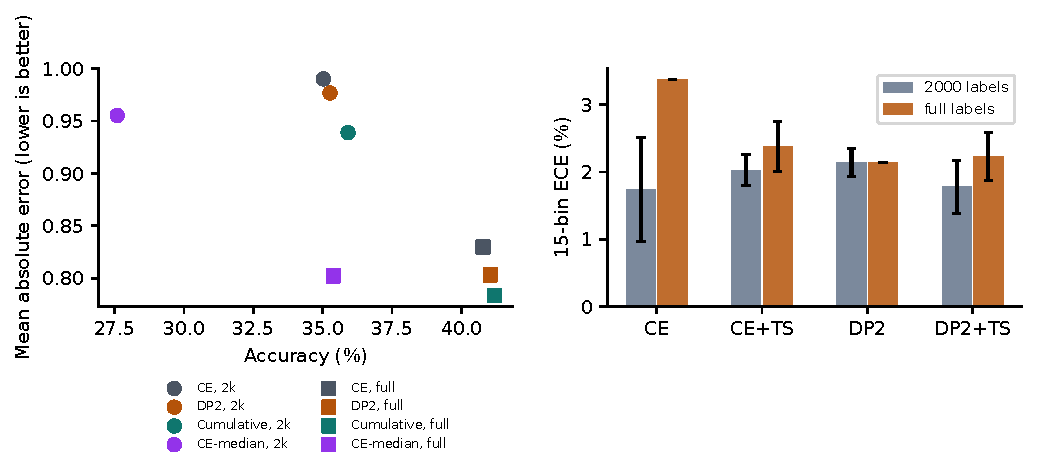
\includegraphics[width=0.95\textwidth]{../figures/tradeoffs.pdf}
\caption{Ordinal prediction and calibration trade-offs computed from saved results. Left: mean accuracy versus MAE for two training budgets. Each plotted point is a run-mean; overlapping scaled decisions are omitted. Right: mean 15-bin ECE with sample standard-deviation bars. A lower ordinal error does not ensure lower calibration error at both budgets.}
\label{fig:tradeoff}
\end{figure*}

\subsection{Calibration changes with the training budget}
Full-budget DP2 has NLL \FullDPtwoNLL{} and ECE \FullDPtwoECE\%, compared with \FullCENLL{} and \FullCEECE\% for CE. CE+TS improves NLL to \FullCETSNLL{} and ECE to \FullCETSECE\%. The full-budget DP2 probability-score advantage remains small when compared with the calibrated baseline rather than raw CE.

The low-budget results in Table~\ref{tab:low} qualify this finding. DP2's MAE is \LowDPtwoMAE{}, compared with \LowCEMAE{} for CE, but its ECE is higher: \LowDPtwoECE\% versus \LowCEECE\%. The hypothesis that distance penalties improve both ordinal error and confidence calibration is therefore not consistently supported. Temperature scaling reduces DP2's low-budget ECE to \LowDPtwoTSECE\%, yet the same transformation slightly increases its full-budget ECE. This is unsurprising because temperatures minimize calibration NLL rather than ECE, and are estimated from a limited sample.

The reliability plot in Figure~\ref{fig:reliability} illustrates the full-budget behavior for seed 42. It is not pooled evidence from independent test sets. High-confidence bins contain relatively few sentences, as shown by the confidence histogram, so visual differences in those bins should not be overinterpreted. ECE rankings also change with the number of bins; the raw quadratic model has lower ECE than raw CE across the tested binnings, but it is not the best method for every bin count.

\begin{table*}[t]
\centering\small
\setlength{\tabcolsep}{5pt}
\begin{tabular}{lrrrrr}
\toprule
Method & Acc. (\%) & MAE & Sev. (\%) & ECE (\%) & NLL \\
\midrule
NB & $34.78\!\pm\!0.47$ & $0.985\!\pm\!0.013$ & $25.08\!\pm\!0.72$ & $2.33\!\pm\!0.30$ & $1.523\!\pm\!0.004$ \\
CE & $35.02\!\pm\!0.61$ & $0.990\!\pm\!0.012$ & $26.05\!\pm\!1.06$ & $1.74\!\pm\!0.77$ & $1.483\!\pm\!0.005$ \\
CE+TS & $35.02\!\pm\!0.61$ & $0.990\!\pm\!0.012$ & $26.05\!\pm\!1.06$ & $2.03\!\pm\!0.23$ & $1.482\!\pm\!0.006$ \\
CE median & $27.60\!\pm\!0.62$ & $0.955\!\pm\!0.005$ & $21.49\!\pm\!0.24$ & $1.74\!\pm\!0.77$ & $1.483\!\pm\!0.005$ \\
Cumulative LR & $35.91\!\pm\!0.09$ & $0.939\!\pm\!0.010$ & $23.09\!\pm\!0.61$ & $1.81\!\pm\!0.44$ & $1.485\!\pm\!0.013$ \\
DP1 & $35.38\!\pm\!0.32$ & $0.976\!\pm\!0.020$ & $25.35\!\pm\!1.46$ & $2.67\!\pm\!0.34$ & $1.479\!\pm\!0.004$ \\
DP2 & $35.26\!\pm\!0.53$ & $0.977\!\pm\!0.017$ & $25.34\!\pm\!1.38$ & $2.14\!\pm\!0.21$ & $1.480\!\pm\!0.004$ \\
DP2+TS & $35.26\!\pm\!0.53$ & $0.977\!\pm\!0.017$ & $25.34\!\pm\!1.38$ & $1.78\!\pm\!0.39$ & $1.479\!\pm\!0.004$ \\
LS & $35.07\!\pm\!0.61$ & $0.989\!\pm\!0.013$ & $26.02\!\pm\!1.08$ & $2.90\!\pm\!0.74$ & $1.487\!\pm\!0.004$ \\
LS+TS & $35.07\!\pm\!0.61$ & $0.989\!\pm\!0.013$ & $26.02\!\pm\!1.08$ & $2.07\!\pm\!0.17$ & $1.481\!\pm\!0.006$ \\
OLL & $35.02\!\pm\!0.59$ & $0.931\!\pm\!0.002$ & $22.14\!\pm\!0.52$ & $10.88\!\pm\!1.08$ & $9.936\!\pm\!0.104$ \\
OLL+TS & $35.02\!\pm\!0.59$ & $0.931\!\pm\!0.002$ & $22.14\!\pm\!0.52$ & $5.67\!\pm\!0.65$ & $1.683\!\pm\!0.003$ \\
\bottomrule
\end{tabular}
\caption{Low-budget results using 2,000 training examples. Run variation now includes sampled training data and development splits. Percent conventions match Table~\ref{tab:main}. The confidence-calibration hypothesis does not hold uniformly.}
\label{tab:low}
\end{table*}

\begin{figure*}[t]
\centering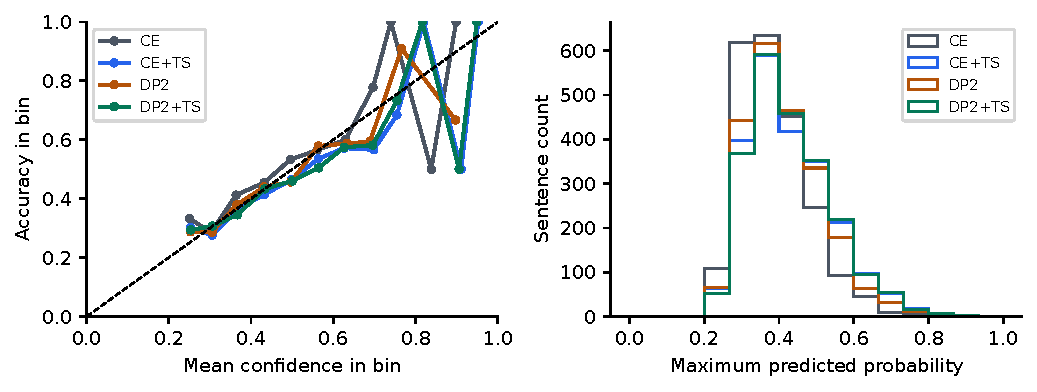
\includegraphics[width=0.94\textwidth]{../figures/reliability.pdf}
\caption{Full-budget reliability diagrams and confidence counts for seed 42. Only nonempty equal-width bins are plotted. Positive temperatures preserve argmax predictions; they can improve NLL while changing binned ECE in either direction.}
\label{fig:reliability}
\end{figure*}

\subsection{Paired evidence and its scope}
Table~\ref{tab:bootstrap} reports conditional paired intervals. DP2's MAE and severe-error differences relative to CE are below zero throughout these intervals. The accuracy interval includes zero, consistent with a small accuracy change. Against the cumulative baseline, DP2 has higher MAE and severe error but lower NLL. We interpret the ordinal benefit over CE as modest evidence within this held-out corpus, not a population-wide or cross-domain result.

\begin{table}[t]
\centering\scriptsize
\setlength{\tabcolsep}{3pt}
\begin{tabular}{llrrr}
\toprule
Reference & Metric & Difference & Lower & Upper \\
\midrule
CE & MAE & -0.027 & -0.041 & -0.013 \\
CE & SEVERE & -1.629 & -2.308 & -0.995 \\
CE & NLL & -0.017 & -0.021 & -0.012 \\
CE & Acc. & 0.271 & -0.543 & 1.086 \\
Cumulative LR & MAE & 0.020 & 0.005 & 0.035 \\
Cumulative LR & SEVERE & 1.493 & 0.769 & 2.262 \\
Cumulative LR & NLL & -0.011 & -0.018 & -0.004 \\
Cumulative LR & Acc. & -0.136 & -1.086 & 0.814 \\
\bottomrule
\end{tabular}
\caption{Full-budget DP2 minus reference: mean paired difference and conditional 95\% bootstrap bounds. Accuracy and severe-error differences are percentage points; MAE and NLL use their original scales. Fitted models are held fixed. The cumulative comparison is secondary.}
\label{tab:bootstrap}
\end{table}

\subsection{Standalone OLL has a probability failure}
The raw OLL baseline obtains MAE \FullOLLMAE{}, but NLL is \FullOLLNLL{} and macro-F1 is \FullOLLFone\%. Figure~\ref{fig:confusion} reveals that it never predicts either extreme class in the representative full-budget fit. Its tail probabilities are extremely small, causing the large NLL even under machine-epsilon clipping. The model can avoid long-distance errors by restricting its decisions to interior labels, while failing to represent the complete class distribution.

This pattern prompted a targeted implementation check. Finite-difference gradients agree with the analytic objective; probability vectors normalize correctly; metric and split audits pass. A constant-input risk diagnostic uses the actual training class proportions rather than an invented dataset. For OLL with exponent one, define $a_k=\sum_y r_y|k-y|$. Minimizing $-\sum_k a_k\log(1-p_k)$ over the probability simplex yields $p_k=\max(0,1-a_k/\nu)$, with $\nu$ chosen so the probabilities sum to one. The executed diagnostic assigns zero mass to both extreme classes. This demonstrates that OLL need not recover class proportions even for a simple constant input. It is consistent with the fitted suppression, although it does not prove the explanation for every sentence.

Temperature scaling lowers OLL's NLL to \FullOLLTSNLL{} but leaves its decisions unchanged. Its fitted temperature reaches the declared upper bound; scaling therefore does not establish a satisfactory calibration repair. These findings are specific to our linear representation, exponent, and optimization setup. They do not invalidate published OLL results with other models or settings.

\begin{figure*}[t]
\centering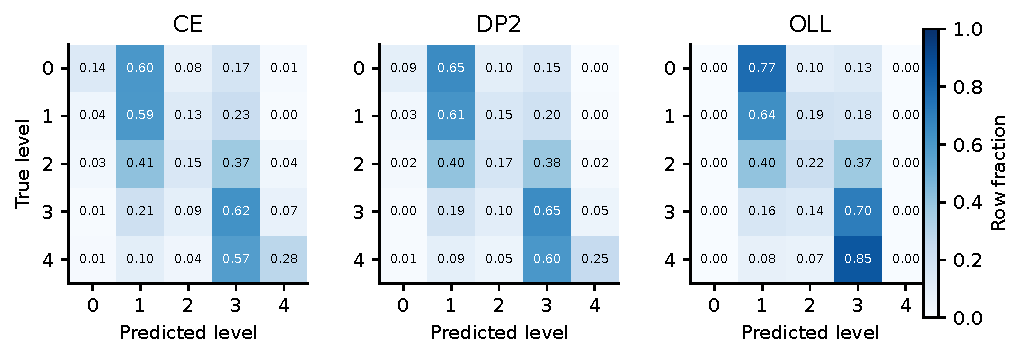
\includegraphics[width=0.95\textwidth]{../figures/confusions.pdf}
\caption{Row-normalized full-budget test confusion matrices for seed 42. DP2 makes somewhat fewer large errors but also fewer extreme-label predictions. OLL predicts only interior levels. The color scale and labels are shared; each row refers to the true class.}
\label{fig:confusion}
\end{figure*}

\subsection{Secondary controls}
Table~\ref{tab:controls} separates the method from some tuning choices. CE-MAE has full-budget MAE \FullCEMAEMAE{}, so matching the ordinal selection criterion does not remove DP2's observed benefit. DP2-NLL selects the same full-budget weight as primary DP2, reproducing its result up to numerical precision. A fixed smaller weight gives MAE \FullDPfixedMAE{}, a weaker improvement. The primary selected weight is at the upper edge of the declared grid. We do not infer a globally optimal weight or expand the grid after seeing test outcomes.

Allowing OLL to choose its own regularization improves raw NLL to \FullOLLregNLL{}, but its accuracy falls to \FullOLLregAcc\%. Temperature scaling gives NLL \FullOLLregTSNLL{}, still worse than the nominal alternatives. Thus a shared regularization strength is a real design limitation, but does not fully explain the observed probability failure. The controls were specified after primary results and are exploratory, rather than independent confirmatory evidence.

\begin{table*}[t]
\centering\small
\setlength{\tabcolsep}{5pt}
\begin{tabular}{lrrrrr}
\toprule
Method & Acc. (\%) & MAE & Sev. (\%) & ECE (\%) & NLL \\
\midrule
CE & $40.77\!\pm\!0.00$ & $0.830\!\pm\!0.000$ & $18.82\!\pm\!0.00$ & $3.37\!\pm\!0.00$ & $1.375\!\pm\!0.000$ \\
CE-MAE & $40.71\!\pm\!0.03$ & $0.829\!\pm\!0.002$ & $18.55\!\pm\!0.47$ & $5.26\!\pm\!3.08$ & $1.381\!\pm\!0.010$ \\
DP2 & $41.04\!\pm\!0.00$ & $0.803\!\pm\!0.000$ & $17.19\!\pm\!0.00$ & $2.14\!\pm\!0.00$ & $1.359\!\pm\!0.000$ \\
DP2-NLL & $41.04\!\pm\!0.00$ & $0.803\!\pm\!0.000$ & $17.19\!\pm\!0.00$ & $2.14\!\pm\!0.00$ & $1.359\!\pm\!0.000$ \\
DP2-fixed & $41.00\!\pm\!0.00$ & $0.822\!\pm\!0.000$ & $18.46\!\pm\!0.00$ & $3.18\!\pm\!0.00$ & $1.369\!\pm\!0.000$ \\
OLL-reg & $30.00\!\pm\!0.00$ & $0.887\!\pm\!0.000$ & $17.24\!\pm\!0.00$ & $8.77\!\pm\!0.00$ & $5.649\!\pm\!0.000$ \\
OLL-reg+TS & $30.00\!\pm\!0.00$ & $0.887\!\pm\!0.000$ & $17.24\!\pm\!0.00$ & $4.45\!\pm\!0.00$ & $1.600\!\pm\!0.000$ \\
\bottomrule
\end{tabular}
\caption{Secondary full-budget controls on the original saved splits. CE-MAE changes CE selection to MAE; DP2-NLL changes penalty selection to NLL; DP2-fixed uses $\lambda=0.5$; OLL-reg tunes its own regularization. These controls address confounds without replacing the primary protocol.}
\label{tab:controls}
\end{table*}

\section{Discussion}
The results distinguish three mechanisms. First, incorporating ordinal costs into training changes the predicted distribution and slightly shifts decisions toward interior labels. Second, a posterior-median action changes ordinal decisions without changing the learned distribution. Third, temperature scaling changes probability quality while preserving argmax classifications. Treating these mechanisms as interchangeable would obscure why a method helps on one metric and harms another.

The additive penalty retains a CE term that rewards probability on the actual label. It therefore avoids the particularly strong tail suppression observed with standalone OLL in this experiment. However, Equation~\ref{eq:distortion} shows why it is not guaranteed to preserve probabilities. The full-budget improvement may arise from a favorable bias in this representation and corpus rather than a general calibration principle. Its low-budget ECE result provides direct evidence against the stronger interpretation.

Classwise inspection also matters. DP2 improves aggregate MAE, but its most-positive-class MAE worsens, and both extreme classes have worse class-conditional NLL than CE. Its lower macro-F1 is consistent with this imbalance. The moderately positive and negative categories form large parts of the corpus; small improvements for frequent interior labels can outweigh harms at the extremes. Consequently, a system that especially values extreme complaints or praise should examine those classes rather than rely only on aggregate distance.

The cumulative baseline is a useful corrective to method-centered conclusions. It performs better on ordinal decisions at both budgets, while DP2 has a better full-budget NLL. The evidence supports choosing a criterion based on the intended use, and considering a simple ordinal model before adding a custom objective. If absolute distance alone determines the downstream action, the posterior median is also a necessary baseline, although its observed accuracy cost is substantial.

Calibration conclusions are similarly metric-dependent. A low ECE can coexist with poor classwise probabilities because ECE summarizes only the confidence of the chosen class. NLL and Brier evaluate the whole distribution, while RPS respects label order through cumulative probabilities. The OLL case makes this distinction particularly clear. The study therefore gives no basis for presenting a single ECE reduction as complete uncertainty improvement.

\section{Limitations and Threats to Validity}
\paragraph{Dataset and representation.} We test one English movie-sentiment corpus at two training budgets. These are not two independent datasets. The experiment cannot establish transfer to product star ratings, code-mixed text, other languages, or domain-shift conditions. Sparse word features miss context, long-range composition, and some negation behavior. Neither the performance level nor the loss ranking should be generalized to pretrained encoders without additional experiments.

\paragraph{Labels and error costs.} Sentiment categories are subjective, and equal spacing is an assumption. A two-level error is our prespecified severity threshold, not a validated application harm measure. Exact normalized deduplication reduces a simple leakage risk but cannot detect all semantic overlap. We do not claim that the official labels are noise-free.

\paragraph{Selection and optimization.} The main objectives share CE's regularization, and DP selects by MAE while CE selects by NLL. Executed secondary controls reduce these confounds, but do not exhaust all objective-specific tuning choices. The selected full-budget penalty lies at a grid boundary. OLL is evaluated at a single exponent; numerical convergence does not guarantee that a nonconvex objective reaches a globally optimal solution. The unpenalized intercept can approach a boundary distribution for OLL.

\paragraph{Uncertainty estimates.} The small development halves limit calibration precision. The full-budget runs share data and often select identical settings, so zero standard deviations are not evidence of broad stability. Bootstrap intervals hold those fitted models fixed and reflect only conditional test-sentence resampling. Numerous secondary metrics and controls are descriptive; we avoid universal significance statements or causal claims.

\paragraph{Reproducibility and practical cost.} Package versions, hardware, settings, splits, model states, and predictions are retained, and every table is generated from saved results. Fit times are recorded for auditing, but this shared-machine run is not a deployment benchmark. The data and the originating publications should be used under their applicable terms. This computational report does not imply faculty supervision, external peer review, or a publication submission.

\section{Conclusion}
We evaluate ordinal training costs and probability calibration together in a reproducible sparse-model sentiment study. The quadratic distance penalty modestly improves full-budget ordinal error and probability scores over CE, but its calibration benefit does not persist at the smaller budget. Cumulative logistic regression produces better ordinal predictions, and posterior-median decisions expose a training-free accuracy--distance trade-off. Standalone OLL has a pronounced probability failure in the tested representation, motivating explicit distribution-level checks. These results support a measured conclusion: ordinal prediction quality and trustworthy probabilities should be tested separately, with matched baselines and clear limits on generalization.

\appendix
\section{Reproduction and Additional Diagnostics}
The repository contains the source PDF extraction, candidate comparison, pretraining protocol hash, amendment log, verified references, analysis, and internal reviewer report. The original dataset archive, processed sentence identifiers, configurations, exact dependency freeze, numerical checks, saved vectorizers and weights, and per-sentence predictions accompany the study. From the repository root, \texttt{uv run --no-sync python -m src.reproduce} replays validation, experiments, secondary controls, analysis, and paper generation after environment setup. Completed runs are resumed from artifacts; a fresh-run option is documented in the README.

The optimizer failure and continuation are preserved rather than removed from the log. A separate audit recomputes final metrics from saved probabilities, checks table macros against those outputs, confirms unchanged TS argmax labels, and checks citation keys. Figures are regenerated from the same files. No test-driven candidate is silently substituted for the validation-selected model.

Additional machine-readable files report all ECE binnings, Brier and ranked probability scores, central prediction fractions, class-conditioned MAE/NLL, and the OLL constant-input risk diagnostic. These supplement the main tables without implying separate dataset replication. They allow readers to examine whether a preferred metric changes the interpretation.

\bibliographystyle{plain}
\bibliography{references}
\end{document}
